% 第15章第1—2节：矩阵逼近问题；秩一逼近（固定方向下的最优系数、Rayleigh商与最优方向、最优解与逼近误差）。

\section{矩阵逼近问题}
\label{sec:matrix-approximation-problem}

数据矩阵常常近似低秩：许多列虽然各不相同，却大致落在少数几个方向张成的子空间里。存储和计算时，我们希望只保留这些方向，用一个秩较低的矩阵代替原矩阵，同时使重建误差尽量小。另一类情形是，某个矩阵按其含义应当正交，例如一次测量得到的旋转，但测量误差使它不再正交；这时要找一个正交矩阵来代替它，并且离测得的矩阵尽量近。

两类问题有共同的形式，称为\term{矩阵逼近}（matrix approximation）。已知矩阵$\bm A\in\mathbb R^{m\times d}$，规定一个允许的矩阵集合$\mathcal X$与一种误差范数，求
\[
 \min_{\bm X\in\mathcal X}\lVert\bm A-\bm X\rVert ,
\]
以及取得最小值的$\bm X$。$\mathcal X$可以是全部秩不超过$k$的矩阵，也可以是全部正交矩阵。

如章首所说，$\bm A$在这里不是方程的系数矩阵：没有右端$\bm b$，也不求输入向量$\bm x$，要输出的是近似矩阵$\bm X$及最小误差。

先采用Frobenius误差。把$\bm A=[\bm a_1,\ldots,\bm a_d]$的列看成$d$个待重建的向量，近似矩阵$\bm X=[\bm x_1,\ldots,\bm x_d]$的列是它们的重建，则
\[
 \lVert\bm A-\bm X\rVert_{\mathrm F}^2=\sum_{j=1}^d\lVert\bm a_j-\bm x_j\rVert_2^2 ,
\]
即各列平方偏差之和。约束$\operatorname{rank}\bm X\leq k$等价于$\bm X$的列空间维数不超过$k$，即全部重建向量共用至多$k$个独立方向。于是秩约束下的问题同时要选两样东西：保留哪些方向，以及每一列在这些方向上取什么系数。

谱范数误差$\lVert\bm A-\bm X\rVert_2$只记录最坏的单位输入方向上的偏差，第~\ref{sec:ls-truncated-svd-optimality}节将比较两种范数下的结论。第~\ref{sec:matrix-approximation-orthogonal}节再把约束换成正交性：那时允许集合不再由秩预算描述，求解方法也随之改变。

取$0\leq k\leq\min(m,d)$，并记$r=\operatorname{rank}\bm A$。两种边界情形可以直接回答：$k=0$时只能取$\bm X=\bm0$，误差为$\lVert\bm A\rVert_{\mathrm F}^2$；$k\geq r$时可以取$\bm X=\bm A$，误差为零，而误差为零又迫使$\bm X=\bm A$。真正需要研究的是$1\leq k<r$。

\begin{example}[三个坐标向量的重建]
\label{ex:ls-low-rank-three-columns}
取$\bm A=[3\bm e_1,2\bm e_2,\bm e_3]$，即$\bm A=\operatorname{diag}(3,2,1)$，三列的长度平方为$9,4,1$，总和$\lVert\bm A\rVert_{\mathrm F}^2=14$。取$k=2$，问题就是用一个过原点的平面重建这三列。把每一列投影到平面上，称投影长度平方之和为保留量，总和中剩下的部分为损失。先比较三个坐标平面：
\begin{itemize}
 \item $\operatorname{span}\{\bm e_1,\bm e_2\}$：保留$9+4=13$，损失$1$；
 \item $\operatorname{span}\{\bm e_1,\bm e_3\}$：保留$9+1=10$，损失$4$；
 \item $\operatorname{span}\{\bm e_2,\bm e_3\}$：保留$4+1=5$，损失$9$。
\end{itemize}
保留最长的两列损失最小。不过这只是三个候选之间的比较：倾斜的平面会同时部分保留三列，它能否比$\operatorname{span}\{\bm e_1,\bm e_2\}$更好，此时还不知道；在平面内取投影是否就是最好的重建，也还需要证明。
\end{example}

示例留下的两个问题，即方向给定时怎样取系数、怎样选方向，下面先在$k=1$时回答（第~\ref{sec:ls-rank-one-rayleigh}节），再推广到一般的$k$（第~\ref{sec:ls-low-rank-approximation}节）。

\section{秩一逼近}
\label{sec:ls-rank-one-rayleigh}

$k=1$时，全部列都用同一个方向的倍数来重建。我们先固定这个方向，求每一列的最优系数；再在全部方向中选出保留平方长度最多的一个。第二步将化成单位向量上的二次型极值问题，它的解由谱分解给出。

\subsection{固定方向下的最优系数}
\label{sec:matrix-approximation-rank-one-coefficients}

先写出全部候选。若$\bm X\neq\bm0$且$\operatorname{rank}\bm X\leq1$，则$\bm X$的列空间是一条直线，由某个非零向量$\bm a$张成，每一列都是$\bm a$的倍数：$\bm x_j=b_j\bm a$，即$\bm X=\bm a\bm b^\top$。令$\bm u=\bm a/\lVert\bm a\rVert_2$、$\bm c=\lVert\bm a\rVert_2\bm b$，就有$\bm X=\bm u\bm c^\top$且$\lVert\bm u\rVert_2=1$。方向的长度可以全部吸收到系数$\bm c$中，所以要求$\bm u$为单位向量不会丢失任何非零候选；$\bm X=\bm0$则对应$\bm c=\bm0$。于是秩不超过一的矩阵恰好是全部$\bm u\bm c^\top$，其中$\lVert\bm u\rVert_2=1$，$\bm c\in\mathbb R^d$。

固定单位方向$\bm u$，第$j$列的重建是$c_j\bm u$。展开平方误差并配方，利用$\bm u^\top\bm u=1$，
\[
 \lVert\bm a_j-c_j\bm u\rVert_2^2
 =\lVert\bm a_j\rVert_2^2-2c_j\bm u^\top\bm a_j+c_j^2
 =\lVert\bm a_j\rVert_2^2-(\bm u^\top\bm a_j)^2+(c_j-\bm u^\top\bm a_j)^2 .
\]
只有最后一项依赖$c_j$，且它非负，所以$c_j=\bm u^\top\bm a_j$是唯一的最优系数，也就是$\bm a_j$在$\bm u$上的正交投影系数。每一列的系数只与该列有关，可以逐列独立求出。合起来写，$\bm c=\bm A^\top\bm u$，最优重建是$\bm u\bm u^\top\bm A$，其中$\bm u\bm u^\top$是到直线$\operatorname{span}\{\bm u\}$的正交投影。

把最优系数代回并对$j$求和，
\[
 \begin{aligned}
 \lVert\bm A-\bm u\bm u^\top\bm A\rVert_{\mathrm F}^2
 &=\lVert\bm A\rVert_{\mathrm F}^2-\sum_{j=1}^d(\bm u^\top\bm a_j)^2\\
 &=\lVert\bm A\rVert_{\mathrm F}^2-\bm u^\top\bm A\bm A^\top\bm u .
 \end{aligned}
\]
称$\bm u^\top\bm A\bm A^\top\bm u$为方向$\bm u$的保留量，它是各列在$\bm u$上投影长度的平方和。总平方长度固定，误差最小等价于保留量最大。于是秩一逼近分成两步：给定方向后，每列做一次内积求出投影系数；再寻找保留量最大的单位方向。后一步由下一小节解决。

\begin{example}[固定方向时的秩一重建]
\label{ex:matrix-approximation-rank-one-fixed-direction}
取
\[
 \bm A=\begin{bmatrix}2&1\\1&2\end{bmatrix},\qquad
 \bm u=\frac1{\sqrt2}\begin{bmatrix}1\\1\end{bmatrix}.
\]
方向固定后，每列的系数就是它在$\bm u$上的投影长度。逐列计算，$c_1=\bm u^\top\bm a_1=(2+1)/\sqrt2=3/\sqrt2$，$c_2=\bm u^\top\bm a_2=(1+2)/\sqrt2=3/\sqrt2$。重建矩阵为
\[
 \bm u\bm c^\top=\frac1{\sqrt2}\cdot\frac3{\sqrt2}\begin{bmatrix}1&1\\1&1\end{bmatrix}
 =\frac32\begin{bmatrix}1&1\\1&1\end{bmatrix},\qquad
 \bm A-\bm u\bm c^\top=\frac12\begin{bmatrix}1&-1\\-1&1\end{bmatrix}.
\]
残差四个元素都是$\pm1/2$，平方和为$1$。也可以不形成残差，用上面的公式核对：$\lVert\bm A\rVert_{\mathrm F}^2=4+1+1+4=10$，保留量$c_1^2+c_2^2=9$，误差$10-9=1$。这个方向是否最好，还要与其他方向比较。
\end{example}

\subsection{Rayleigh商与最优方向}
\label{sec:ls-quadratic-extrema}
\label{sec:ls-rayleigh-extremal}

上一小节把选方向化成：在单位向量中最大化$\bm u^\top\bm G\bm u$，其中$\bm G=\bm A\bm A^\top$对称半正定。同样的问题对一般的实对称矩阵$\bm S$也会出现：第~\ref{sec:linear-algebra-homogeneous-estimation}节的齐次最小二乘要在单位向量中求二次型的最小值，第~\ref{chap:condition-and-spectral-perturbation}章比较扰动前后的特征值时也要用到这类极值。所以下面先对任意实对称$\bm S$回答：输入方向改变时，二次型$\bm x^\top\bm S\bm x$最大、最小能取到多少，在哪些方向取到？然后再回到$\bm G$。

先看最简单的对角矩阵$\bm S=\operatorname{diag}(4,1)$，此时$\bm x^\top\bm S\bm x=4x_1^2+x_2^2$。固定$\bm x^\top\bm x=1$，比较不同单位方向上的值：第一坐标方向$\bm e_1$给出$4$，第二坐标方向$\bm e_2$给出$1$。看起来最大值是$4$、最小值是$1$，但这只比较了两个候选。单位圆上还有无穷多个倾斜方向，例如$(1,1)^\top/\sqrt2$给出$5/2$；要证明全局极值，必须对所有单位方向都作出比较。

长度约束的作用是让比较只关注方向。二次型随$\bm x$的长度按平方增长：若不加约束，把$\bm e_2$放大到$3\bm e_2$，二次型就变成$9$，超过了$\bm e_1$方向的值，这只反映了输入被放大，与方向无关。把长度除掉，就得到只依赖方向的量，称为\term{Rayleigh商}（Rayleigh quotient）。
\begin{definition}[Rayleigh商]
\label{def:matrix-analysis-rayleigh-quotient}
对实对称矩阵$\bm S\in\mathbb R^{d\times d}$与$\bm x\neq\bm0$，
\begin{equation}
 R_{\bm S}(\bm x)=\frac{\bm x^\top\bm S\bm x}{\bm x^\top\bm x}.
 \label{eq:matrix-analysis-rayleigh-quotient}
\end{equation}
\end{definition}
把$\bm x$换成$c\bm x$（$c\neq0$）时分子分母同乘$c^2$，Rayleigh商不变，所以它只依赖$\bm x$所在的直线。对任意$\bm x\neq\bm0$，$R_{\bm S}(\bm x)$等于单位向量$\bm x/\lVert\bm x\rVert_2$上的二次型值；反过来，单位向量上的二次型值就是它的Rayleigh商。因此求Rayleigh商在全部非零向量上的极值，等价于在单位球面上求二次型的极值。

谱分解把这种比较化为对特征值的比较。按第~\ref{sec:ls-symmetric-spectral-decomposition}节的约定，把$\bm S$的特征值排成$\lambda_1\geq\cdots\geq\lambda_d$，对应标准正交特征向量$\bm q_1,\ldots,\bm q_d$。对单位向量$\bm x=\sum_ic_i\bm q_i$，有$\sum_ic_i^2=\lVert\bm x\rVert_2^2=1$，由二次型展开式~\eqref{eq:matrix-analysis-quadratic-spectral-form}，
\[
 R_{\bm S}(\bm x)=\sum_{i=1}^d\lambda_ic_i^2 .
\]
它是各特征值以$c_i^2$为权的加权平均：权重非负，总和为$1$。加权平均介于被平均各数的最小值与最大值之间，由此得到两端特征值的极值刻画。

\begin{theorem}[Rayleigh--Ritz]
\label{thm:matrix-analysis-rayleigh-ritz}
设$\bm S\in\mathbb R^{d\times d}$对称，特征值为$\lambda_1\geq\cdots\geq\lambda_d$，对应标准正交特征向量$\bm q_1,\ldots,\bm q_d$。则对一切$\bm x\neq\bm0$，
\begin{equation}
 \lambda_d\leq R_{\bm S}(\bm x)\leq\lambda_1 ,
 \label{eq:matrix-analysis-rayleigh-ritz}
\end{equation}
于是$\max_{\bm x\neq\bm0}R_{\bm S}(\bm x)=\lambda_1$，$\min_{\bm x\neq\bm0}R_{\bm S}(\bm x)=\lambda_d$，分别在$\bm q_1$与$\bm q_d$取到。进一步，$R_{\bm S}(\bm x)=\lambda_1$当且仅当$\bm x$是$\ker(\bm S-\lambda_1\bm I)$中的非零向量；$R_{\bm S}(\bm x)=\lambda_d$当且仅当$\bm x$是$\ker(\bm S-\lambda_d\bm I)$中的非零向量。
\end{theorem}
\begin{proof}
Rayleigh商不随缩放改变，只需对单位向量$\bm x=\sum_ic_i\bm q_i$证明。这时$R_{\bm S}(\bm x)=\sum_i\lambda_ic_i^2$且$\sum_ic_i^2=1$，所以
\[
 \lambda_1-R_{\bm S}(\bm x)=\sum_{i=1}^d(\lambda_1-\lambda_i)c_i^2\geq0 ,
\]
每一项都非负。同理$R_{\bm S}(\bm x)-\lambda_d=\sum_i(\lambda_i-\lambda_d)c_i^2\geq0$。这就是式~\eqref{eq:matrix-analysis-rayleigh-ritz}。取$\bm x=\bm q_1$时$c_1=1$、其余$c_i=0$，得$R_{\bm S}(\bm q_1)=\lambda_1$；取$\bm x=\bm q_d$得$\lambda_d$。所以两端的界都能取到。

再看取等条件。上面的和式等于零，当且仅当每一项都为零，即凡$\lambda_i<\lambda_1$的$i$都有$c_i=0$。这恰好说明$\bm x$落在满足$\lambda_i=\lambda_1$的那些$\bm q_i$的张成中；由定理~\ref{thm:ls-spectral-projections}，这个张成就是特征空间$\ker(\bm S-\lambda_1\bm I)$。最小值的情形相同。
\end{proof}

图~\ref{fig:ls-sphere-constrained-extremum}用一个二阶对称矩阵画出这一关系：二次型的水平椭圆在特征方向处与单位圆相切，切点处取到极值。

\begin{figure}[htbp]
  \centering
  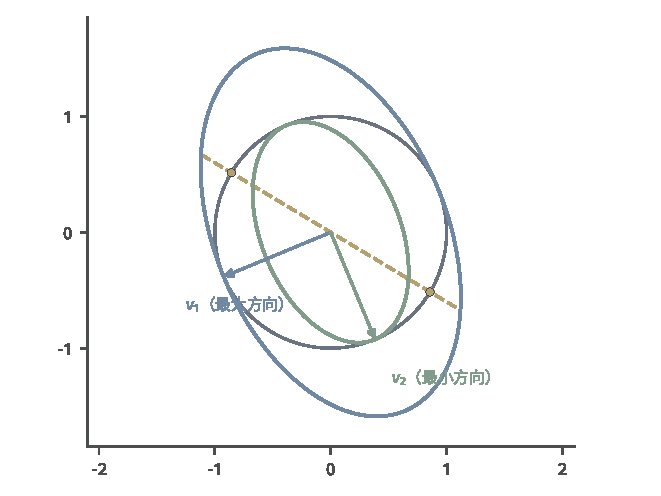
\includegraphics[width=112mm]{figures/00-shared/mathematical-preliminaries-upper/02-linear-spaces/matplotlib/ls-sphere-constrained-extremum/ls-sphere-constrained-extremum.pdf}
  \caption{单位圆约束下的极值落在特征方向。$\bm S=\left[\begin{smallmatrix}2&0.5\\0.5&1\end{smallmatrix}\right]$，
  灰圆为$\lVert\bm x\rVert=1$。蓝椭圆$\bm x^\top\bm S\bm x=\lambda_1\approx2.21$在
  $\pm\bm v_1$处与单位圆相切（最大值），绿椭圆$=\lambda_2\approx0.79$在$\pm\bm v_2$处
  相切（最小值）；黄色虚线为子空间约束直线，其上黄点是该约束下的两个极值，
  第~\ref{sec:ls-spectral-value-sensitivity}节的最小最大原理使用这种限制。
  $\lambda_{1,2}=(3\pm\sqrt2)/2$。固定复算。}
  \label{fig:ls-sphere-constrained-extremum}
\end{figure}

回到开头的对角矩阵，现在可以完成全部单位方向的比较。

\begin{example}[对角矩阵在全部单位方向上的比较]
\label{ex:ls-rayleigh-diagonal-two-by-two}
取$\bm S=\operatorname{diag}(4,1)$。每个单位向量都能写成$\bm x=(\cos\theta,\sin\theta)^\top$，其中$\theta\in[0,2\pi)$，于是
\[
 \bm x^\top\bm S\bm x=4\cos^2\theta+\sin^2\theta=1+3\cos^2\theta .
\]
由$0\leq\cos^2\theta\leq1$，它介于$1$与$4$之间：$\cos^2\theta=1$即$\bm x=\pm\bm e_1$时取最大值$4$，$\cos^2\theta=0$即$\bm x=\pm\bm e_2$时取最小值$1$。

可见最大值$4$与最小值$1$正是两个特征值，取到它们的方向正是特征方向，与定理~\ref{thm:matrix-analysis-rayleigh-ritz}一致；倾斜方向的值都严格介于两者之间。
\end{example}

定理不要求$\bm S$半正定。二次型可以取负值，例如$\bm S=\operatorname{diag}(1,-2)$时$\bm x^\top\bm S\bm x=x_1^2-2x_2^2$，单位方向上的值仍介于$-2$与$1$之间，两端分别在$\pm\bm e_2$与$\pm\bm e_1$取到。

还要区分最优值与最优方向的唯一性。最大值$\lambda_1$总是唯一的数，取到它的方向则由特征空间$\ker(\bm S-\lambda_1\bm I)$决定。$\lambda_1$单重时，这个空间是一条直线，单位最优方向只有$\pm\bm q_1$两个，相差一个符号；$\lambda_1$重复时，空间中每个单位向量都给出最大值，例如$\bm S=\bm I$时所有单位方向都是最优的。

重根时，谱分解中的$\bm q_1$只是最优方向中的一个代表，取决于特征基的选择；最优方向组成的集合则由定理~\ref{thm:ls-spectral-projections}唯一确定。最小值的情形相同。

一个常见的特例是$\bm S=\bm A^\top\bm A$，其中$\bm A\in\mathbb R^{m\times d}$。这时
\[
 R_{\bm A^\top\bm A}(\bm x)=\frac{\bm x^\top\bm A^\top\bm A\bm x}{\bm x^\top\bm x}=\frac{\lVert\bm A\bm x\rVert_2^2}{\lVert\bm x\rVert_2^2},
\]
即输出长度与输入长度之比的平方。第~\ref{chap:singular-value-decomposition}章已经说明$\bm A^\top\bm A$的特征值是奇异值的平方（$d>m$时补上零），所以定理~\ref{thm:matrix-analysis-rayleigh-ritz}给出那里最大、最小输出长度的另一种解释：单位输入的输出长度最大为$\sigma_1$，在$\bm v_1$取到；最小为$\sqrt{\lambda_d}$，其中$\lambda_d$是$\bm A^\top\bm A$的最小特征值，在它的特征方向取到。

第~\ref{sec:linear-algebra-homogeneous-estimation}节的齐次最小二乘正是在单位输入中最小化这一量。若$\bm A$有非零的零空间，最小值为零，任一单位零空间向量都最优；若$\bm A$满列秩，则$\bm A\bm x\neq\bm0$对一切$\bm x\neq\bm0$成立，$\bm A^\top\bm A\succ0$，由定理~\ref{thm:ls-symmetric-definiteness-eigenvalues}，最小值为正。

现在回到秩一逼近，取$\bm S=\bm G=\bm A\bm A^\top$。由定理~\ref{thm:matrix-analysis-rayleigh-ritz}，单位方向的保留量$\bm u^\top\bm G\bm u$最大为$\lambda_1(\bm G)$，恰在$\ker(\bm G-\lambda_1(\bm G)\bm I)$中的单位向量处取到，最小平方误差为$\lVert\bm A\rVert_{\mathrm F}^2-\lambda_1(\bm G)$。这里只使用了第~\ref{chap:eigen-spectral-decomposition}章已经证明的谱分解；谱分解的存在不依赖本节的极值结论，本节只是用它读出极值。

\begin{example}[比较两个特征方向]
\label{ex:matrix-approximation-rank-one-eigen-directions}
沿用示例~\ref{ex:matrix-approximation-rank-one-fixed-direction}的$\bm A$，
\[
 \bm G=\bm A\bm A^\top=\begin{bmatrix}5&4\\4&5\end{bmatrix}.
\]
$\bm G(1,1)^\top=9(1,1)^\top$，$\bm G(1,-1)^\top=(1,-1)^\top$，所以两个标准正交特征方向$(1,1)^\top/\sqrt2$与$(1,-1)^\top/\sqrt2$的保留量分别是$9$与$1$。前者给出重建平方误差$10-9=1$，后者给出$10-1=9$。由定理~\ref{thm:matrix-analysis-rayleigh-ritz}，任何单位方向的误差都介于$1$与$9$之间，所以示例~\ref{ex:matrix-approximation-rank-one-fixed-direction}所取的方向已是最优方向，而$(1,-1)^\top/\sqrt2$是最差的方向。
\end{example}

\subsection{最优解与逼近误差}
\label{sec:matrix-approximation-rank-one-solution}

上一小节用$\bm G$的特征方向给出了最优直线，现在把它与$\bm A$的奇异值分解联系起来，写出最优近似矩阵。设$\bm A\neq\bm0$，奇异值为$\sigma_1\geq\cdots\geq\sigma_r>0$。式~\eqref{eq:ls-svd-transpose-relation}说明，$\bm G=\bm A\bm A^\top$的特征值是$\sigma_1^2,\ldots,\sigma_r^2$及$m-r$个零，左奇异向量$\bm u_i$是对应的特征向量。因此最大保留量为$\lambda_1(\bm G)=\sigma_1^2$，取$\bm u=\bm u_1$即可达到，最小平方误差为$\lVert\bm A\rVert_{\mathrm F}^2-\sigma_1^2=\sum_{i=2}^r\sigma_i^2$。

再由$\bm A^\top\bm u_1=\sigma_1\bm v_1$，最优系数是$\bm c=\bm A^\top\bm u_1=\sigma_1\bm v_1$，“最佳方向加最优系数”合成
\[
 \bm A_1=\bm u_1\bm u_1^\top\bm A=\bm u_1(\bm A^\top\bm u_1)^\top=\sigma_1\bm u_1\bm v_1^\top .
\]
这是原矩阵$\bm A$的秩一近似，即和式~\eqref{eq:matrix-analysis-svd-rank-one-sum}的第一项，而不是Gram矩阵$\bm G$的秩一近似。计算的输入是$\bm A$及其已经求出的SVD，输出是近似矩阵$\bm A_1$；它不是某个方程的系数向量。

具体计算依次是：读取最大奇异值$\sigma_1$及配对的方向$\bm u_1$、$\bm v_1$，作外积$\bm u_1\bm v_1^\top$并乘以$\sigma_1$，最后求残差$\bm A-\bm A_1$并核对误差。沿用示例~\ref{ex:matrix-approximation-rank-one-fixed-direction}，$\bm A$对称正定，$\bm A(1,1)^\top=3(1,1)^\top$，$\bm A(1,-1)^\top=(1,-1)^\top$，所以$\sigma_1=3$、$\sigma_2=1$，可取$\bm u_1=\bm v_1=(1,1)^\top/\sqrt2$。于是
\[
 \bm A_1=3\cdot\frac12\begin{bmatrix}1&1\\1&1\end{bmatrix}=\frac32\begin{bmatrix}1&1\\1&1\end{bmatrix},
\]
四个元素都是$3/2$，两列成比例，秩为一；残差与示例~\ref{ex:matrix-approximation-rank-one-fixed-direction}相同，Frobenius范数为$1=\sigma_2$。在示例~\ref{ex:ls-low-rank-three-columns}中，$\bm G=\operatorname{diag}(9,4,1)$，最佳直线是$\bm e_1$方向，保留量$9$，损失$5$；重建$3\bm e_1\bm e_1^\top$只保留第一列，另两列被投影成零。

这里用的是$\bm A\bm A^\top$而不是$\bm A^\top\bm A$，因为我们重建的是$\mathbb R^m$中的列向量，保留量直接等于列向量在$\bm u$上的投影长度平方之和，对应的是左奇异方向。若改为重建行向量，同样的推导会用到$\bm A^\top\bm A$与右奇异方向$\bm v_1$，得到的近似$\bm A\bm v_1\bm v_1^\top=\sigma_1\bm u_1\bm v_1^\top$是同一个矩阵。

这种解释依赖$\bm G$是Gram矩阵。对一般不定的对称矩阵$\bm S$，二次型值可能为负，不能把任意Rayleigh商的极值都解释成某个矩阵的最佳秩一逼近。

最后区分最优近似矩阵与它的表示。$\bm A=\bm0$时$r=0$，每个方向的保留量都是零，唯一的最优近似是零矩阵。$\sigma_1>\sigma_2$（或$r=1$）时，$\bm G$最大特征值的特征空间是一条直线，最优方向只有$\pm\bm u_1$；把$(\bm u_1,\bm v_1)$同时换成$(-\bm u_1,-\bm v_1)$不改变外积，所以最优矩阵$\bm A_1$唯一，不唯一的只是它的写法。

$\sigma_1=\sigma_2$时情况不同：最大特征值的特征空间至少二维，其中每个单位向量$\bm u$都给出最优近似$\bm u\bm u^\top\bm A$，不同的直线给出不同的矩阵。例如$\bm A=\bm I_2$时，$\bm e_1\bm e_1^\top$与$\bm e_2\bm e_2^\top$的平方误差都是$1$。所以表示的非唯一性不等于近似矩阵的非唯一性，后者只来自最大奇异值重复。下一步保持误差标准不变，把允许保留的方向数由一个增加到$k$个。
